\documentclass{beamer}
\usepackage[T1]{fontenc}
\usepackage{lmodern}
\usefonttheme{serif}

\title{Statistische Inferenz und Kausalität}
\subtitle{Interventionen}
\author{-}
\date{14.07.2023}

\usetheme{Warsaw}
\usecolortheme{seahorse}

\usepackage[utf8]{inputenc}
\usepackage{amsmath,amsfonts,amsthm,amssymb}
\usepackage[ngerman]{babel}
\usepackage{float}
\usepackage{tikz}
\usepackage{xcolor}
\usepackage{hyperref}
\usepackage{doi}
\usepackage{graphicx}
\usepackage{helvet}

\usepackage{listings}

\definecolor{codegreen}{rgb}{0,0.6,0}
\definecolor{codegray}{rgb}{0.5,0.5,0.5}
\definecolor{codepurple}{rgb}{0.58,0,0.82}
\definecolor{backcolour}{rgb}{0.95,0.95,0.92}

\lstdefinestyle{mystyle}{
    backgroundcolor=\color{backcolour},   
    commentstyle=\color{codegreen},
    keywordstyle=\color{magenta},
    numberstyle=\tiny\color{codegray},
    stringstyle=\color{codepurple},
    basicstyle=\ttfamily\footnotesize,
    breakatwhitespace=false,         
    breaklines=true,                 
    captionpos=b,                    
    keepspaces=true,                 
    numbers=left,                    
    numbersep=5pt,                  
    showspaces=false,                
    showstringspaces=false,
    showtabs=false,                  
    tabsize=2
}

\lstset{style=mystyle}
\usepackage{enumitem}

\newcommand{\en}[1]{{\scriptsize(\textit{#1})}}
\newcommand{\kom}[1]{\ignorespaces}
\newcommand{\red}[1]{{\color{red}#1}}
\newcommand{\green}[1]{{\color{green}#1}}
\newcommand{\Cov}{\operatorname{Cov}}
\newcommand{\Do}{\operatorname{do}}
\newcommand{\ACE}{\operatorname{ACE}}
\newcommand{\Pa}{\operatorname{Pa}}
\newcommand{\pa}{\operatorname{pa}}
\newcommand{\Bild}{\operatorname{Im}}
\newcommand{\Poiss}{\operatorname{Poiss}}
\newcommand{\klein}[1]{{\scriptsize #1}}

\tikzstyle{endo} = [rectangle, draw, fill=white, minimum size=2em]
\tikzstyle{invis} = [draw=none]

\AtBeginSection[]
{
\begin{frame}
\frametitle{Inhaltsverzeichnis}
\tableofcontents[currentsection]
\end{frame}
}

\setbeamertemplate{headline}{}

\begin{document}
\frame{\titlepage}

\section{Einführung}
\begin{frame}
\frametitle{Einführung}

Ziel der kausalen Inferenz: Wirkungen mögliche Ursachen zuordnen.

\vspace*{\baselineskip}
\pause

Die \textit{kausale Hierarchie} \en{causal hierarchy} ist gegeben durch.
\begin{enumerate}[label=(\roman*)]
\item Assoziation
\item Intervention
\item Kontrafaktisches
\end{enumerate}
\end{frame}

\section{Wiederholung}
\begin{frame}
\frametitle{Bedingte Wahrscheinlichkeit und bedingte Erwartung}

\begin{block}{\textbf{Definition 4.1} \klein{(Bedingte Wahrscheinlichkeit und bedingte Erwartung)}}
Seien $X$ und $Y$ messbare Zufallsvariablen mit Werten $x$ und $y$. Sei weiter $\mathbb{P}(Y = y) > 0$. Dann ist die \textit{bedingte Wahrscheinlichkeit} von $X = x$ unter der Bedingung $Y = y$ definiert durch
\[\mathbb{P}(X = x \mid Y = y) := \frac{\mathbb{P}(X = x, Y = y)}{\mathbb{P}(Y = y)}~.\]
\pause
Seien $x_1, \dots, x_n$ alle Werte von $X$. Dann ist die \textit{bedingte Erwartung} von $X$ unter der Bedingung $Y = y$ definiert durch
\[\mathbb{E}(X \mid Y = y) := \sum_{i=1}^n x_i \mathbb{P}(X = x_i \mid Y = y)~.\]
\end{block}
\end{frame}

\begin{frame}
\frametitle{Stochastische Unabhängigkeit}

\begin{block}{\textbf{Definition 4.2} \klein{(Stochastische Unabhängigkeit)}}
Seien $X$ und $Y$ messbare Zufallsvariablen. $X$ und $Y$ heißen \textit{stochastische unabhängig}, wenn für alle Kombinationen von Werten $x$ von $X$ und $y$ von $Y$ gilt
\[\mathbb{P}(X = x, Y = y) = \mathbb{P}(X = x) \cdot \mathbb{P}(Y = y)~.\]
\end{block}

\pause

Sind $X$ und $Y$ unabhängig, so gilt
\[\mathbb{P}(X = x \mid Y = y) = \mathbb{P}(X = x)~.\]
\end{frame}

\begin{frame}
\frametitle{Satz von der totalen Wahrscheinlichkeit}

\begin{block}{\textbf{Satz 4.5} \klein{(Satz von der totalen Wahrscheinlichkeit)}}
Seien $X$ und $Y$ messbare Zufallsvariablen. Sei $x$ ein Wert von $X$ und $y_1, \dots, y_n$ alle Werte von $Y$. Dann gilt folgende Zerlegung
\[\mathbb{P}(X = x) = \sum_{i=1}^n \mathbb{P}(X = x \mid Y = y_i) \cdot \mathbb{P}(Y = y_i)~.\]
\end{block}
\end{frame}

\begin{frame}
\frametitle{Kausal- und Korrelationsgraph}

\begin{block}{\textbf{Definition 4.6} \klein{(Kausal- und Korrelationsgraph)}}
Ein \textit{Kausalgraph} \en{SCM} ist ein gerichteter, azyklischer Graph. Die Knoten des Graphen beschreiben die betrachteten Variablen und die Pfeile dazwischen die Richtung des kausalen Zusammenhangs.\\
\pause
Ein \textit{Korrelationsgraph} ist ein ungerichteter Graph. Die Knoten des Graphen beschreiben wieder die betrachteten Variablen und die Linien dazwischen die Assoziationen der Variablen.
\end{block}
\end{frame}

\begin{frame}
\frametitle{Exogene und endogene Variablen}

\begin{block}{\textbf{Definition 4.9} (Exogene und endogene Variablen)}
\textit{Exogene Variablen} \en{exogenous variables} sind Variablen, deren Werte außerhalb eines gegebenen Modells bestimmt werden, womit darauf kein Einfluss genommen werden kann. Sie werden als gegeben und unabhängig von allen anderen Variablen angenommen. Bezeichnet werden die Variablen mit $U_X, U_Y, U_Z, \dots$ und ihre Werte mit $u_X, u_Y, u_Z, \dots$.\\
\pause
\textit{Endogene Variablen} \en{endogenous variables} sind Variablen, die durch Zustände, die im Modell stattfindet und durch die exogenen Variablen bestimmt werden. Bezeichnet werden die Variablen mit $X, Y, Z, \dots$ und ihre Werte mit $x, y, z, \dots$.\\
Wir setzen voraus, dass wir endogene Variablen also Funktionen von anderen Variablen.
\end{block}
\end{frame}

\begin{frame}
\frametitle{Pflanzenwachstum}

\begin{columns}[b]
\begin{column}{0.5\linewidth}
\begin{align*}
W &=~\text{Wasser}\\
L &=~\text{Licht}\\
G &=~\text{Größer}
\end{align*}

\begin{center}
\begin{tikzpicture}[->,>=stealth,shorten >=1pt,auto,node distance=2cm,semithick]  
  \node (U_X) {$U_G$};
  \node (U_Y) [right of=U_X] {$U_W$};
  \node (U_{Y, Z}) [right of=U_Y] {$U_{W, L}$};
  \node[invis] (H) [below of=U_X] {};
  \node[endo] (Y) [below of=U_Y] {$W$};
  \node[endo] (Z) [below of=U_{Y, Z}] {$L$};
  \node[endo] (X) [below of=H] {$G$};

  \path (U_{Y, Z}) edge node {} (Z);
  \path (U_{Y, Z}) edge node {} (Y);
  \path (U_Y) edge node {} (Y);
  \path (U_X) edge node {} (X);
  \path (Z) edge node {} (X);
  \path (Y) edge node {} (X);
\end{tikzpicture}
\end{center}
\end{column}
\begin{column}{0.5\linewidth}
\[G = f_G(W, L, U_G)\]
\pause
\begin{center}
\begin{tikzpicture}[->,>=stealth,shorten >=1pt,auto,node distance=2cm,semithick]  
  \node (U_X) {$U_G$};
  \node[invis] (U_Y) [right of=U_X] {$w$};
  \node (U_{Y, Z}) [right of=U_Y] {$U_{W, L}$};
  \node[invis] (H) [below of=U_X] {};
  \node[endo] (Y) [below of=U_Y] {$W = w$};
  \node[endo] (Z) [below of=U_{Y, Z}] {$L$};
  \node[endo] (X) [below of=H] {$G$};

  \path (U_{Y, Z}) edge node {} (Z);
  \path (U_Y) edge node {} (Y);
  \path (U_X) edge node {} (X);
  \path (Z) edge node {} (X);
  \path (Y) edge node {} (X);
\end{tikzpicture}
\end{center}
\end{column}
\end{columns}
\end{frame}

\section{Kausalität und Korrelation}

\begin{frame}
\frametitle{Kausalität}

\begin{block}{\textbf{Definition 4.12} \klein{Kausalität}}
Seien $X$ und $Y$ Zufallsvariablen. Wir sagen $X$ \textit{verursacht} $Y$ \en{cause}\kom{S. 5}, wenn die Werte von $Y$ in irgendeiner Weise von den Werten von $X$ abhängen.
\end{block}

\pause
\vspace*{3\baselineskip}

\begin{center}
\begin{tikzpicture}[->,>=stealth,shorten >=1pt,auto,node distance=2cm,semithick]  
  \node (X) {$X$};
  \node (Y) [right of=X] {$Y$};

  \path (X) edge node {} (Y);
\end{tikzpicture}
\end{center}
\end{frame}

\begin{frame}
\frametitle{Korrelation}

\begin{block}{\textbf{Definition 4.16} \klein{Korrelation}}
Seien $X$ und $Y$ Zufallsvariablen. Wir sagen $X$ und $Y$ sind \textit{korreliert} \en{correlated}\kom{S. 22}, wenn ihre \textit{Kovarianz} nicht verschwindet. Es soll also gelten
\[\Cov(X, Y) = \mathbb{E}(XY) - \mathbb{E}(X) \mathbb{E}(Y) \neq 0~.\]
Man sagt auch $X$ und $Y$ sind \textit{assoziiert}.
\end{block}

\pause
\vspace*{2\baselineskip}

\begin{center}
\begin{tikzpicture}[-,>=stealth,shorten >=1pt,auto,node distance=2cm,semithick]  
  \node (X) {$X$};
  \node (Y) [right of=X] {$Y$};

  \path (X) edge node {} (Y);
\end{tikzpicture}
\end{center}
\end{frame}

\begin{frame}
\frametitle{Kausalprinzip}

\begin{block}{Kausalprinzip}
Seien $X$ und $Y$ assoziierte Variablen. Dann gilt das \textit{Kausalprinzip} und somit eine der folgenden Aussagen.
\begin{enumerate}[label=(\roman*)]
\item $X$ folgt aus $Y$
\item $Y$ folgt aus $X$
\item Es gibt ein $Z$ mit $X$ folgt aus $Z$ und $Y$ folgt aus $Z$
\end{enumerate}
\end{block}

\pause

\begin{columns}
\begin{column}{0.33\linewidth}
\begin{center}
\begin{tikzpicture}[->,>=stealth,shorten >=1pt,auto,node distance=2cm,semithick]  
  \node (X) {$X$};
  \node (Y) [right of=X] {$Y$};

  \path (Y) edge node {} (X);
\end{tikzpicture}
\end{center}
\end{column}
\begin{column}{0.33\linewidth}
\begin{center}
\begin{tikzpicture}[->,>=stealth,shorten >=1pt,auto,node distance=2cm,semithick]  
  \node (Y) {$Y$};
  \node (X) [right of=Y] {$X$};

  \path (X) edge node {} (Y);
\end{tikzpicture}
\end{center}
\end{column}
\begin{column}{0.33\linewidth}
\begin{center}
\begin{tikzpicture}[->,>=stealth,shorten >=1pt,auto,node distance=2cm,semithick]  
  \node (Z) {$Z$};
  \node (X) [below left of=Z] {$X$};
  \node (Y) [below right of=Z] {$Y$};

  \path (Z) edge node {} (X);
  \path (Z) edge node {} (Y);
\end{tikzpicture}
\end{center}
\end{column}
\end{columns}
\end{frame}

\begin{frame}
\frametitle{Eisverkauf}

Sei $E$ die Anzahl der Eisverkäufe und $D$ die Anzahl der Taschendiebstähle.

\begin{tiny}
\begin{center}
\begin{tabular}{| l | c | c | c | c | c | c | c | c | c | c | c |}
\hline
$E$ & $1860$ & $1985$ & $2211$ & $2215$ & $2712$ & $2387$ & $2801$ & $2912$ & $3058$ & $3032$ & $2812$\\
\hline
$D$ & $10$ & $12$ & $11$ & $15$ & $17$ & $18$ & $20$ & $19$ & $22$ & $21$ & $23$\\
\hline
\end{tabular}
\end{center}
\end{tiny}

\pause

\begin{center}
	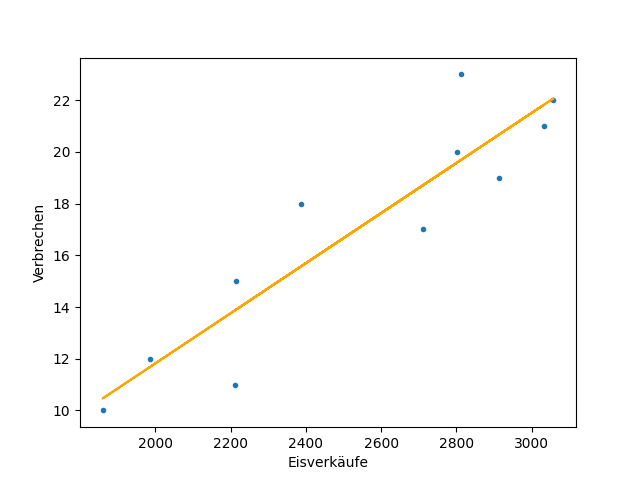
\includegraphics[width=0.5\linewidth]{Eisverkäufe vs Taschendiebstähle.png}
\end{center}
\end{frame}

\begin{frame}
\frametitle{Eisverkauf}

Sei $T$ die Temperatur.

\begin{tiny}
\begin{center}
\begin{tabular}{| l | c | c | c | c | c | c | c | c | c | c | c |}
\hline
$T$ & $18$ & $20$ & $21$ & $23$ & $24$ & $25$ & $27$ & $28$ & $29$ & $30$ & $32$\\
\hline
$E$ & $1860$ & $1985$ & $2211$ & $2215$ & $2712$ & $2387$ & $2801$ & $2912$ & $3058$ & $3032$ & $2812$\\
\hline
$D$ & $10$ & $12$ & $11$ & $15$ & $17$ & $18$ & $20$ & $19$ & $22$ & $21$ & $23$\\
\hline
\end{tabular}
\end{center}
\end{tiny}

\pause
\vspace*{-\baselineskip}

\begin{columns}
\begin{column}{0.5\linewidth}
\begin{center}
	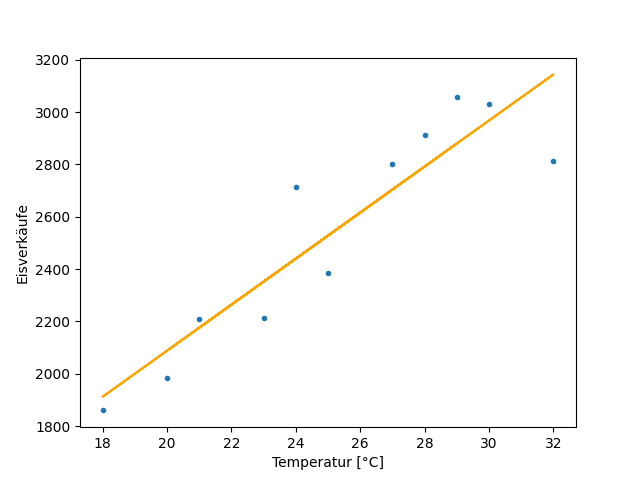
\includegraphics[width=1.1\linewidth]{Temperatur vs Eisverkäufe.png}
\end{center}
\end{column}
\begin{column}{0.5\linewidth}
\begin{center}
	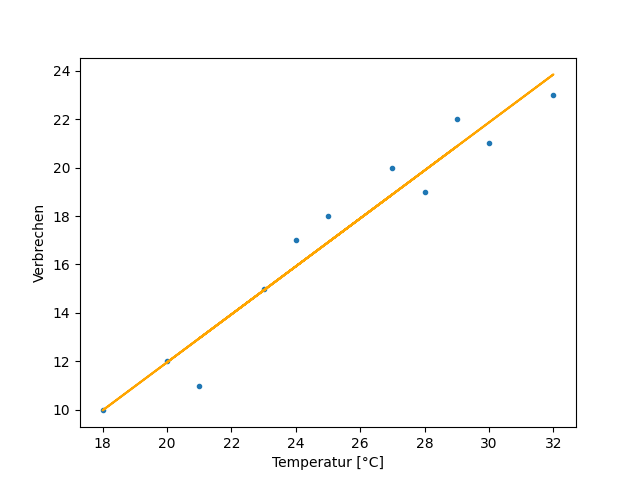
\includegraphics[width=1.1\linewidth]{Temperatur vs Taschendiebstähle.png}
\end{center}
\end{column}
\end{columns}
\end{frame}

\begin{frame}
\frametitle{Eisverkauf}

\begin{center}
\begin{tikzpicture}[->,>=stealth,shorten >=1pt,auto,node distance=2cm,semithick]
  \node (U_X) {$U_T$};  
  \node[endo] (X) [below of=U_X] {$T$};
  \node[endo] (Y) [below left of=X] {$E$};
  \node[endo] (Z) [below right of=X] {$D$};
  \node (U_Y) [above of=Y] {$U_E$};
  \node (U_Z) [above of=Z] {$U_D$};

  \path (U_X) edge node {} (X);
  \path (U_Y) edge node {} (Y);
  \path (U_Z) edge node {} (Z);
  \path (X) edge node {} (Y);
  \path (X) edge node {} (Z);
\end{tikzpicture}
\end{center}
\end{frame}

\section{Interventionen}

\begin{frame}
\frametitle{Intervention}

\begin{block}{\textbf{Definition 4.19} \klein{(Intervention)}}
Sei $X$ eine Zufallsvariable und $x \in \Bild(X)$ einer ihrer Werte. Eine \textit{Intervention} ist eine Maßnahme, um den Wert der Zufallsvariable auf $x$ zu fixieren. Dies schreiben wir als $\Do(X = x)$.
\end{block}

\pause
\vspace*{2\baselineskip}

\textit{Lokalität}: Intervention hat keine Nebenwirkungen.
\end{frame}

\begin{frame}
\frametitle{Pflanzenwachstum}
\begin{columns}
\begin{column}{0.5\linewidth}
\begin{center}
\begin{tikzpicture}[->,>=stealth,shorten >=1pt,auto,node distance=2cm,semithick]  
  \node (U_X) {$U_G$};
  \node (U_Y) [right of=U_X] {$U_W$};
  \node (U_{Y, Z}) [right of=U_Y] {$U_{W, L}$};
  \node[invis] (H) [below of=U_X] {};
  \node[endo] (Y) [below of=U_Y] {$W$};
  \node[endo] (Z) [below of=U_{Y, Z}] {$L$};
  \node[endo] (X) [below of=H] {$G$};

  \path (U_{Y, Z}) edge node {} (Z);
  \path (U_{Y, Z}) edge node {} (Y);
  \path (U_Y) edge node {} (Y);
  \path (U_X) edge node {} (X);
  \path (Z) edge node {} (X);
  \path (Y) edge node {} (X);
\end{tikzpicture}
\end{center}
\end{column}
\begin{column}{0.5\linewidth}
\begin{center}
\begin{tikzpicture}[->,>=stealth,shorten >=1pt,auto,node distance=2cm,semithick]  
  \node (U_X) {$U_G$};
  \node[invis] (U_Y) [right of=U_X] {$w$};
  \node (U_{Y, Z}) [right of=U_Y] {$U_{W, L}$};
  \node[invis] (H) [below of=U_X] {};
  \node[endo] (Y) [below of=U_Y] {$W = w$};
  \node[endo] (Z) [below of=U_{Y, Z}] {$L$};
  \node[endo] (X) [below of=H] {$G$};

  \path (U_{Y, Z}) edge node {} (Z);
  \path (U_Y) edge node {} (Y);
  \path (U_X) edge node {} (X);
  \path (Z) edge node {} (X);
  \path (Y) edge node {} (X);
\end{tikzpicture}
\end{center}
\end{column}
\end{columns}
\end{frame}

\begin{frame}
\frametitle{Eisverkauf}

Präintervention
\begin{tiny}
\begin{center}
\begin{tabular}{| l | c | c | c | c | c | c | c | c | c | c | c |}
\hline
$E$ & $1860$ & $1985$ & $2211$ & $2215$ & $2712$ & $2387$ & $2801$ & $2912$ & $3058$ & $3032$ & $2812$\\
\hline
$D$ & $10$ & $12$ & $11$ & $15$ & $17$ & $18$ & $20$ & $19$ & $22$ & $21$ & $23$\\
\hline
\end{tabular}
\end{center}
\end{tiny}

\[\mathbb{E}(D \mid E \leq 2500) \approx 13.2\]

\pause

Postintervention
\begin{tiny}
\begin{center}
\begin{tabular}{| l | c | c | c | c | c | c | c | c | c | c | c |}
\hline
$E$ & $1864$ & $1992$ & $2221$ & $2315$ & $2500$ & $2387$ & $2500$ & $2500$ & $2500$ & $2500$ & $2500$\\
\hline
$D$ & $10$ & $11$ & $10$ & $15$ & $18$ & $18$ & $19$ & $20$ & $21$ & $21$ & $24$\\
\hline
\end{tabular}
\end{center}
\end{tiny}

\[\mathbb{E}(D \mid \Do(E \leq 2500)) \approx 17.1\]
\end{frame}

\begin{frame}
\frametitle{Eisverkauf}

\begin{center}
\begin{tikzpicture}[->,>=stealth,shorten >=1pt,auto,node distance=2cm,semithick]
  \node (U_X) {$U_T$};  
  \node[endo] (X) [below of=U_X] {$T$};
  \node[endo] (Y) [below left of=X] {$E \leq 2500$};
  \node[endo] (Z) [below right of=X] {$D$};
  \node (U_Z) [above of=Z] {$U_D$};
  \node (U_Y) [above of=Y] {$\leq 2500$};

  \path (U_X) edge node {} (X);
  \path (U_Z) edge node {} (Z);
  \path (U_Y) edge node {} (Y);
  \path (X) edge node {} (Z);
\end{tikzpicture}
\end{center}
\end{frame}

\begin{frame}
\frametitle{Randomisierte kontrollierte Studie}

\begin{center}
	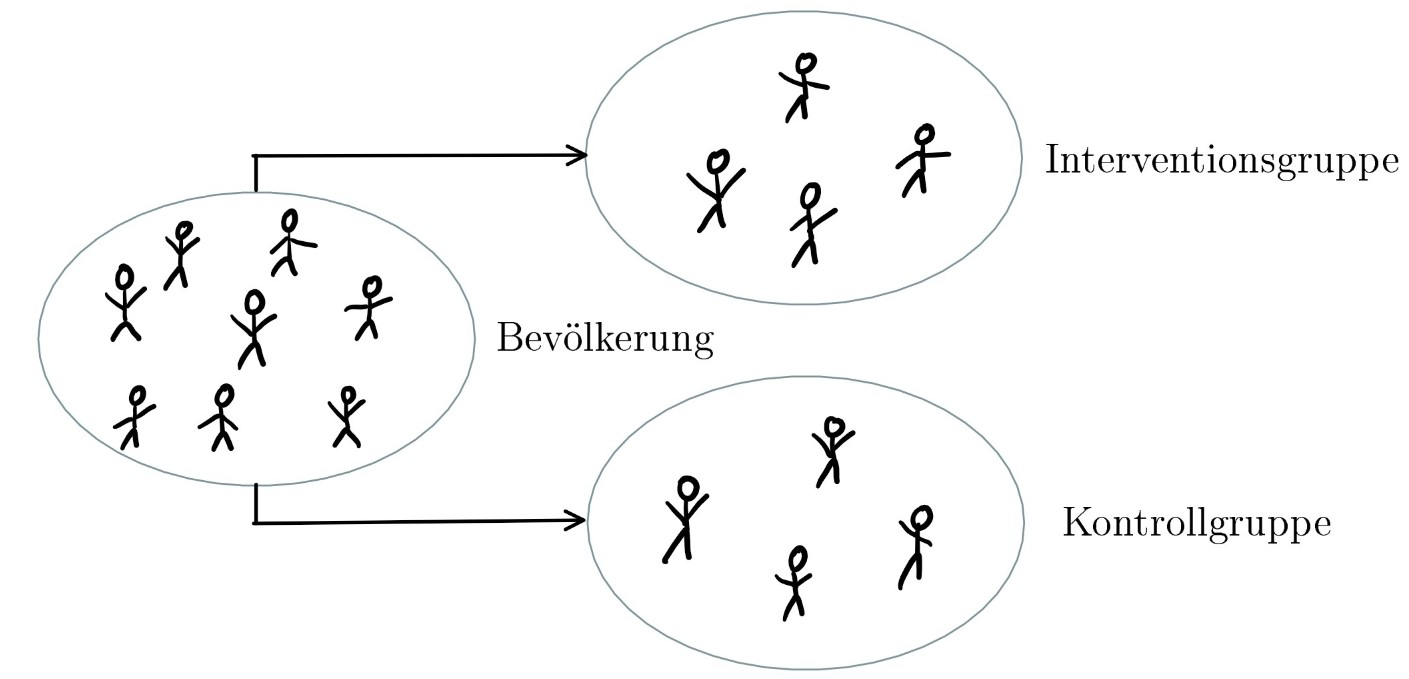
\includegraphics[width=0.9\linewidth]{Randomisierte_Kontrollierte_Studie.jpg}
\end{center}
\end{frame}

\begin{frame}
\frametitle{Unterschied Konditionierung und Intervention}

Seien $X$ und $Y$ Zufallsvariablen und $y$ ein Wert von $Y$.\\

$\mathbb{P}(X = \cdot \mid Y = y)$ ist die Verteilung von $X$ unter der Teilmenge der Individuen mit $Y = y$.\\

\vspace*{\baselineskip}
\pause

$\mathbb{P}(X = \cdot \mid \Do(Y = y))$ ist die Verteilung von $X$ unter einer Bevölkerung, die ausschließlich $Y = y$ besitzt.
\end{frame}

\section{Adjustierungsformel}

\begin{frame}
\frametitle{Durchschnittlicher kausaler Effekt}

\begin{block}{\textbf{Definition 4.25} \klein{(Durchschnittlicher kausaler Effekt)}}
Seien $X$ und $Y$ Variablen und $X$ sogar \textit{binär}, habe also nur die Werte $0$ und $1$. Wir definieren den \textit{durchschnittlichen kausalen Effekt von $X$ auf $Y$} ($\ACE$) \en{average causal effect, causal effect difference} durch
\[\ACE(X \rightarrow Y) := \mathbb{P}(Y = y \mid \Do(X = 1)) - \mathbb{P}(Y = y \mid \Do(X = 0))~.\]
\end{block}
\end{frame}

\begin{frame}
\frametitle{Simpson Paradoxon}

Beschreibe $M$ die Gabe des Medikaments, $G$ das Geschlecht und $H$ die Heilung.

\begin{columns}
\begin{column}{0.7\linewidth}
\begin{scriptsize}
\begin{center}
\begin{tabular}{| c | c | c |}
\hline
& $M = 0$ & $M = 1$\\
\hline
$G = 0$ & $55$ von $80$ ($69 \%$) & $192$ von $263$ ($73 \%$)\\
\hline
$G = 1$ & $234$ von $270$ ($87 \%$) & $81$ von $87$ ($93 \%$)\\
\hline
Gesamt & $289$ von $350$ ($83 \%$) & $273$ von $350$ ($78 \%$)\\
\hline
\end{tabular}
\end{center}
\end{scriptsize}
\end{column}

\pause

\begin{column}{0.3\linewidth}
\begin{center}
\begin{scriptsize}
\begin{tikzpicture}[->,>=stealth,shorten >=1pt,auto,node distance=1.25cm,semithick]
  \node (H_eins) {};
  \node (U_Z) [right of=H_eins] {$U_G$};
  \node (H_zwei) [right of=U_Z] {};
  \node (U_X) [below of=H_eins] {$U_M$};
  \node[endo] (Z) [below of=U_Z] {$G$};
  \node (U_Y) [below of=H_zwei] {$U_H$};
  \node[endo] (X) [below of=U_X] {$M$};
  \node[endo] (Y) [below of=U_Y] {$H$};
  
  \path (U_X) edge node {} (X);
  \path (U_Y) edge node {} (Y);
  \path (U_Z) edge node {} (Z);
  \path (Z) edge node {} (X);
  \path (Z) edge node {} (Y);
  \path (X) edge node {} (Y);
\end{tikzpicture}
\end{scriptsize}
\end{center}
\end{column}
\end{columns}
\end{frame}

\begin{frame}
\frametitle{Simpson Paradoxon}

Naiv
\[\mathbb{P}(H = 1 \mid M = 1) - \mathbb{P}(H = 1 \mid M = 0) = - 5 \%~.\]

\pause

Paradox, weil
\begin{align*}
\mathbb{P}(H = 1 \mid G = 0, M = 1) &> \mathbb{P}(H = 1 \mid G = 0, M = 0)
\intertext{und}
\mathbb{P}(H = 1 \mid G = 1, M = 1) &> \mathbb{P}(H = 1 \mid G = 1, M = 0)~.
\end{align*}

\pause

Daher
\[\ACE(M \rightarrow H) = \mathbb{P}(H = 1 \mid \Do(M = 1)) - \mathbb{P}(H = 1 \mid \Do(M = 0))~.\]
\end{frame}

\begin{frame}
\frametitle{Simpson Paradoxon}

Intervention zur Auflösung von $G \rightarrow M$.

\begin{center}
\begin{tikzpicture}[->,>=stealth,shorten >=1pt,auto,node distance=2cm,semithick]
  \node (H_eins) {};
  \node (U_Z) [right of=H_eins] {$U_G$};
  \node (H_zwei) [right of=U_Z] {};
  \node (U_X) [below of=H_eins] {$m$};
  \node[endo] (Z) [below of=U_Z] {$G$};
  \node (U_Y) [below of=H_zwei] {$U_H$};
  \node[endo] (X) [below of=U_X] {$M = m$};
  \node[endo] (Y) [below of=U_Y] {$H$};
  
  \path (U_X) edge node {} (X);
  \path (U_Y) edge node {} (Y);
  \path (U_Z) edge node {} (Z);
  \path (Z) edge node {} (Y);
  \path (X) edge node {} (Y);
\end{tikzpicture}
\end{center}
\end{frame}

\begin{frame}
\frametitle{Simpson Paradoxon}

Die noch zu zeigende Adjustierungsformel liefert
\begin{align*}
\mathbb{P}(H = 1 \mid \Do(M = 1)) &= \mathbb{P}(H = 1 \mid M = 1, G = 0) \mathbb{P}(G = 0)\\
&+ \mathbb{P}(H = 1 \mid M = 1, G = 1) \mathbb{P}(G = 1)\\
&= 73 \% \cdot \frac{263 + 80}{700} + 93 \% \cdot \frac{87 + 270}{700}\\
&= 35.77 \% + 47.43 \% = 83.2 \%
\intertext{und}
\mathbb{P}(H = 1 \mid \Do(M = 0)) &= \mathbb{P}(D = 1 \mid M = 0, G = 0) \mathbb{P}(G = 0)\\
&+ \mathbb{P}(H = 1 \mid M = 0, G = 1) \mathbb{P}(G = 1)\\
&= 69 \% \cdot \frac{263 + 80}{700} + 87 \% \cdot \frac{87 + 270}{700}\\
&= 33.81 \% + 44.37 \% = 78.18 \%~.
\end{align*}
\end{frame}

\begin{frame}
\frametitle{Simpson Paradoxon}

Daraus erhalten wir
\begin{align*}
\ACE(M \rightarrow H) &= \mathbb{P}(H = 1 \mid \Do(M = 1))\\
&- \mathbb{P}(H = 1 \mid \Do(M = 0))\\
&= 5.02 \%~.
\end{align*}

Entspricht der Intuition.
\end{frame}

\begin{frame}
\frametitle{Adjustierungsformel}

\begin{block}{\textbf{Satz 4.27} \klein{(Adjustierungsformel)}}
Seien $X$, $Y$ und $Z$ Zufallsvariablen, sodass $Z$ eine Ursache für $X$ und $Y$ ist. Weiter sei $Y$ noch eine Folge von $X$. Außerdem sei $x$ ein Wert von $X$ und $y$ ein Wert von $Y$. Nach der \textit{Adjustierungsformel} \en{adjustment formula} gilt dann
\begin{small}
\[\mathbb{P}(Y = y \mid \Do(X = x)) = \sum_{z \in \Bild(Z)} \mathbb{P}(Y = y \mid X = x, Z = z) \cdot \mathbb{P}(Z = z)~.\]
\end{small}
\end{block}
\end{frame}

\begin{frame}
\frametitle{Blutdruck}

Beschreibe $M$ die Gabe des Medikaments, $B$ den Blutdruck nach Gabe des Medikaments / Placebos und $H$ die Heilung.

\begin{columns}
\begin{column}{0.7\linewidth}
\begin{scriptsize}
\begin{center}
\begin{tabular}{| c | c | c |}
\hline
& $M = 0$ & $M = 1$\\
\hline
$B = 0$ & $81$ von $87$ ($93 \%$) & $234$ von $270$ ($87 \%$)\\
\hline
$B = 1$ & $192$ von $263$ ($73 \%$) & $55$ von $80$ ($69 \%$)\\
\hline
Gesamt & $273$ von $350$ ($78 \%$) & $289$ von $350$ ($83 \%$)\\
\hline
\end{tabular}
\end{center}
\end{scriptsize}
\end{column}
\pause
\begin{column}{0.3\linewidth}
\begin{center}
\begin{scriptsize}
\begin{tikzpicture}[->,>=stealth,shorten >=1pt,auto,node distance=1.25cm,semithick]
  \node (H_eins) {};
  \node (U_Z) [right of=H_eins] {$U_B$};
  \node (H_zwei) [right of=U_Z] {};
  \node (U_X) [below of=H_eins] {$U_M$};
  \node[endo] (Z) [below of=U_Z] {$B$};
  \node (U_Y) [below of=H_zwei] {$U_H$};
  \node[endo] (X) [below of=U_X] {$M$};
  \node[endo] (Y) [below of=U_Y] {$H$};
  
  \path (U_X) edge node {} (X);
  \path (U_Y) edge node {} (Y);
  \path (U_Z) edge node {} (Z);
  \path (X) edge node {} (Z);
  \path (Z) edge node {} (Y);
  \path (X) edge node {} (Y);
\end{tikzpicture}
\end{scriptsize}
\end{center}
\end{column}
\end{columns}

\pause

Da $M$ bis auf $U_M$ keine Eltern hat, gilt
\[\mathbb{P}(H = h \mid \Do(M = m)) = \mathbb{P}(H = h \mid M = m)~.\]
\end{frame}

\section{Die Regel vom kausalen Effekt}

\begin{frame}
\frametitle{Die Regel vom kausalen Effekt}

\begin{block}{\textbf{Satz 4.30} \klein{(Die Regel vom kausalen Effekt)}}
Sei ein Kausalgraph gegeben und $\Pa(X)$ der Zufallsvektor der Eltern von $X$, sowie $Y$ eine weiter Zufallsvariable. Dann gilt für den kausalen Effekt von $X$ auf $Y$
\begin{scriptsize}
\[\mathbb{P}(Y = y \mid \Do(X = x)) = \sum_{z \in \Bild(\Pa(X))} \mathbb{P}(Y = y \mid X = x, \Pa(X) = z) \cdot \mathbb{P}(\Pa(X) = z)~.\]
\end{scriptsize}
Hierbei seien $y$ und $x$ Werte von $Y$ respektive $X$ und $z$ ein mögliche Kombination von Werten des Vektors $\Pa(X)$.
\end{block}
\end{frame}

\begin{frame}
\frametitle{Blutdruck und Geschlecht}

Beschreibe $M$ die Gabe des Medikaments, $G$ das Geschlecht, $B$ den Blutdruck nach Gabe des Medikaments / Placebos und $H$ die Heilung.

\pause

\begin{center}
\begin{tikzpicture}[->,>=stealth,shorten >=1pt,auto,node distance=2cm,semithick]
  \node (U_G) {$U_G$};
  \node (G) [right of=U_G] {$G$};
  \node (B) [right of=G] {$B$};
  \node (U_B) [right of=B] {$U_B$};
  \node (U_H) [below of=U_G] {$U_H$};
  \node (H) [right of=U_H] {$H$};
  \node (M) [right of=H] {$M$};
  \node (U_M) [right of=M] {$U_M$};
  
  \path (U_G) edge node {} (G);
  \path (U_B) edge node {} (B);
  \path (U_H) edge node {} (H);
  \path (U_M) edge node {} (M);
  \path (G) edge node {} (B);
  \path (G) edge node {} (M);
  \path (G) edge node {} (H);
  \path (B) edge node {} (H);
  \path (M) edge node {} (H);
  \path (M) edge node {} (B);
\end{tikzpicture}
\end{center}
\end{frame}

\begin{frame}
\frametitle{Blutdruck und Geschlecht}

\begin{scriptsize}
\begin{center}
\begin{tabular}{| c | c | c |}
\hline
& $M = 0$ & $M = 1$\\
\hline
$G = 0$ & $128$ von $500$ ($26 \%$) & $372$ von $500$ ($74 \%$)\\
\hline
$G = 1$ & $52$ von $500$ ($10 \%$) & $448$ von $500$ ($90 \%$)\\
\hline
\end{tabular}
\end{center}
\end{scriptsize}

\begin{scriptsize}
\begin{align*}
\mathbb{P}(H = 1 \mid B = 0, G = 0, M = 0) &= 15 \%\\
\mathbb{P}(H = 1 \mid B = 0, G = 1, M = 0) &= 16 \%\\
\mathbb{P}(H = 1 \mid B = 0, G = 0, M = 1) &= 53 \%\\
\mathbb{P}(H = 1 \mid B = 0, G = 1, M = 1) &= 42 \%~.
\end{align*}
\end{scriptsize}

\pause

Mit $\Pa(B) = \{G, M, U_B\}$ folgt mit der Regel vom kausalen Effekt
\begin{scriptsize}
\begin{align*}
\mathbb{P}(H = 1 \mid \Do(B = 0)) &= \sum_{z \in \{0, 1\}^2} \mathbb{P}(H = 1 \mid B = 0, G = g, M = m) \cdot \mathbb{P}(G = g, M = m)\\
&\approx 83 \%~.
\end{align*}
\end{scriptsize}
\end{frame}

\begin{frame}
\frametitle{Poissonverteilung}

\begin{columns}
\begin{column}{0.3\linewidth}
\begin{scriptsize}
Sei
\begin{align*}
U_V &\sim \Poiss(5)\\
U_W &\sim \Poiss(5)\\
U_X &\sim \Poiss(3)\\ 
U_Y &\sim \Poiss(1)\\
U_Z &\sim \Poiss(1)
\end{align*}
und
\begin{align*}
V &:= U_V\\
W &:= U_W\\
X &:= V + U_X\\
Y &:= V + W + X + U_Y\\
Z &:= X + Y + U_Z~.
\end{align*}
\end{scriptsize}
\end{column}

\pause

\begin{column}{0.7\linewidth}
\begin{center}
\begin{tikzpicture}[->,>=stealth,shorten >=1pt,auto,node distance=1.5cm,semithick]
  \node (U_X) {$U_X$};
  \node (U_V) [right of=U_X] {$U_V$};
  \node (U_W) [right of=U_V] {$U_W$};
  \node[endo] (X) [below of=U_X] {$X$};
  \node[endo] (V) [below of=U_V] {$V$};
  \node[endo] (W) [below of=U_W] {$W$};
  \node[endo] (Z) [below of=X] {$Z$};
  \node[endo] (Y) [below of=V] {$Y$};
  \node (U_Z) [below of=Z] {$U_Z$};
  \node (U_Y) [below of=Y] {$U_Y$};
  
  \path (U_V) edge node {} (V);
  \path (U_W) edge node {} (W);
  \path (U_X) edge node {} (X);
  \path (U_Y) edge node {} (Y);
  \path (U_Z) edge node {} (Z);
  \path (V) edge node {} (X);
  \path (V) edge node {} (Y);
  \path (W) edge node {} (Y);
  \path (X) edge node {} (Y);
  \path (X) edge node {} (Z);
  \path (Y) edge node {} (Z);
\end{tikzpicture}
\end{center}
\end{column}
\end{columns}
\end{frame}

\begin{frame}
\frametitle{Poissonverteilung}

\begin{columns}
\begin{column}{0.33\linewidth}
\begin{center}
	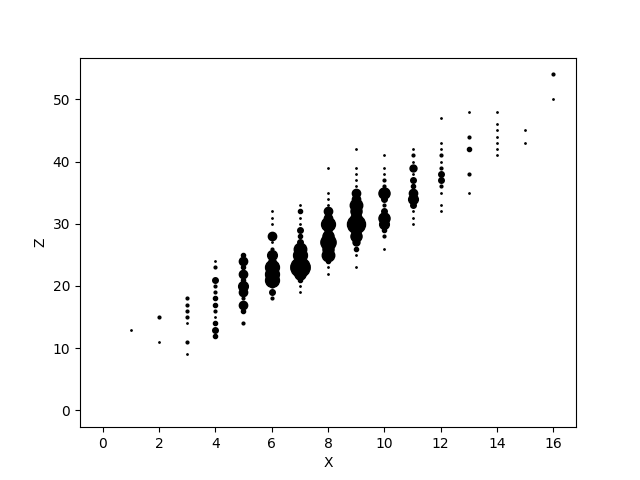
\includegraphics[width=1.1\linewidth]{X_Z_Poiss_Pre.png}
\end{center}
\end{column}
\begin{column}{0.33\linewidth}
\begin{center}
	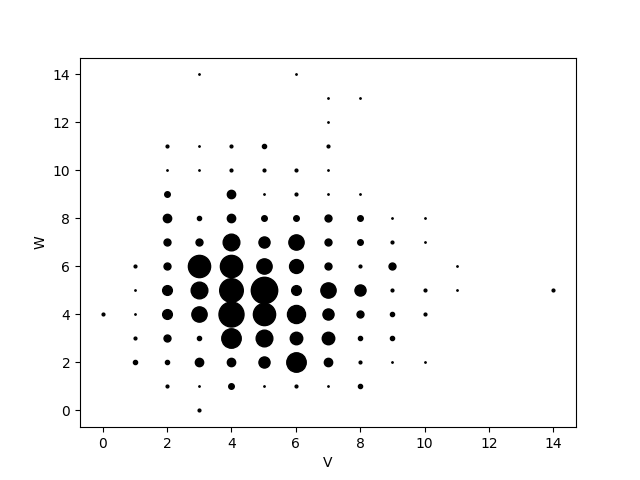
\includegraphics[width=1.1\linewidth]{V_W_Poiss_Pre.png}
\end{center}
\end{column}
\begin{column}{0.33\linewidth}
\begin{center}
	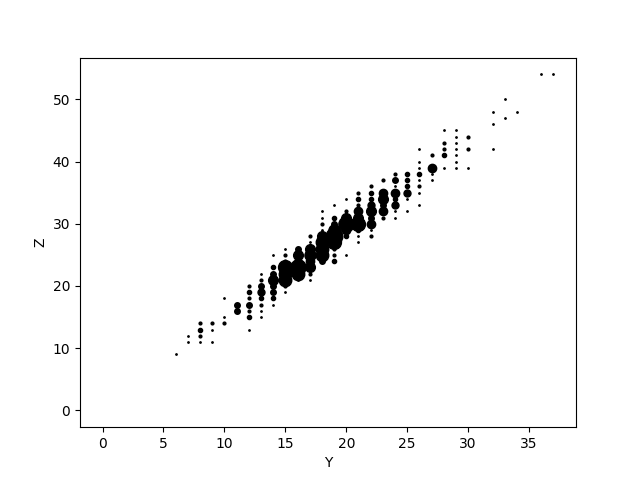
\includegraphics[width=1.1\linewidth]{Y_Z_Poiss_Pre.png}
\end{center}
\end{column}
\end{columns}

\begin{columns}
\begin{column}{0.33\linewidth}
\begin{center}
	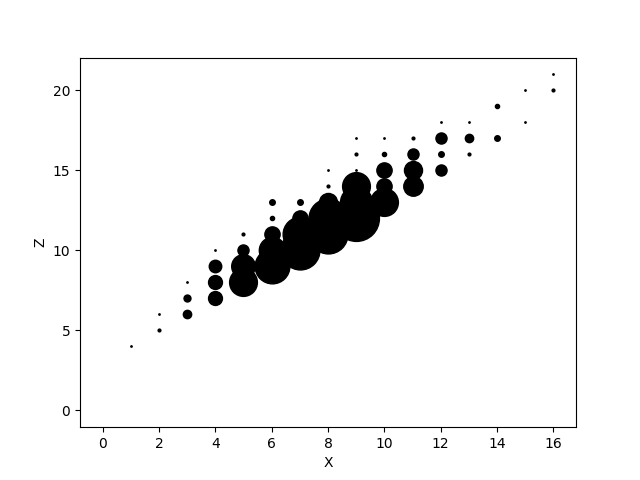
\includegraphics[width=1.1\linewidth]{X_Z_Poiss_Post.png}
\end{center}
\end{column}
\begin{column}{0.33\linewidth}
\begin{center}
	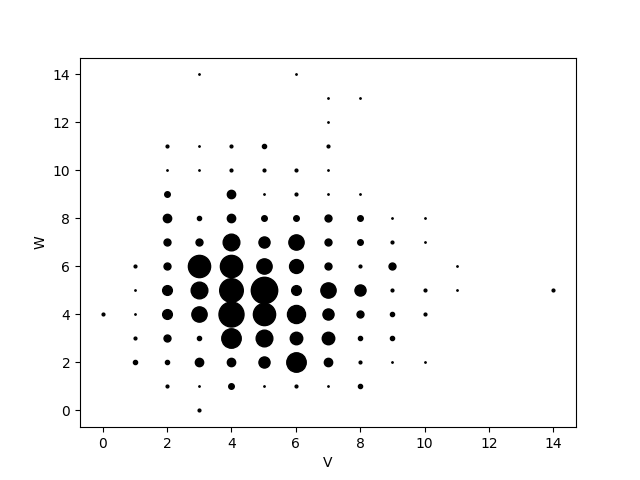
\includegraphics[width=1.1\linewidth]{V_W_Poiss_Post.png}
\end{center}
\end{column}
\begin{column}{0.33\linewidth}
\begin{center}
	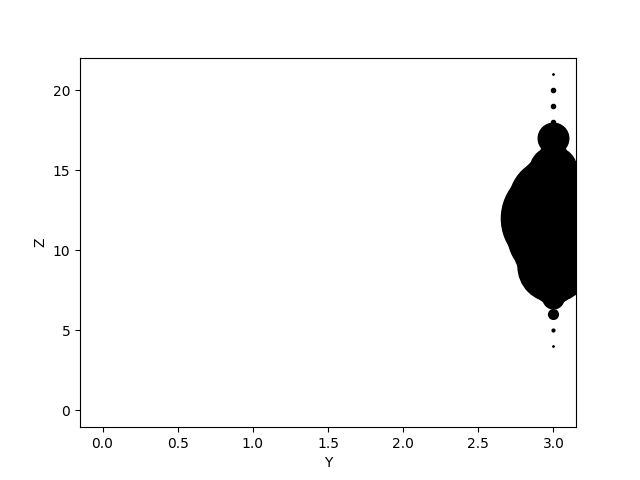
\includegraphics[width=1.1\linewidth]{Y_Z_Poiss_Post.png}
\end{center}
\end{column}
\end{columns}
\end{frame}

\begin{frame}
\frametitle{Poissonverteilung}

Die Regel vom kausalen Effekt liefert
\begin{small}
\begin{align*}
\mathbb{P}(Z = z \mid \Do(Y = y)) = \sum_{(v, w, x) \in \mathbb{N}_0^3}& \mathbb{P}(Z = z \mid Y = y, V = v, W = w, X = x)\\
&\cdot \mathbb{P}(V = v, W = w, X = x)~.
\end{align*}
\end{small}

Nach einer Simulation für $Z = 10$ und $Y = 3$ ist dies ungefähr $12 \%$.
\end{frame}

\begin{frame}
\frametitle{Normalverteilung}

\begin{columns}
\begin{column}{0.3\linewidth}
\begin{scriptsize}
Sei
\begin{align*}
U_V &\sim \mathcal{N}(0, 1)\\
U_W &\sim \mathcal{N}(0, 2)\\
U_X &\sim \mathcal{N}(0, 1)\\ 
U_Y &\sim \mathcal{N}(0, 0.1)\\
U_Z &\sim \mathcal{N}(0, 0.2)
\end{align*}
und
\begin{align*}
V &:= U_V\\
W &:= U_W\\
X &:= W + U_X\\
Y &:= W + X + U_Y\\
Z &:= V + Y + U_Z~.
\end{align*}
\end{scriptsize}
\end{column}

\pause

\begin{column}{0.7\linewidth}
\begin{center}
\begin{tikzpicture}[->,>=stealth,shorten >=1pt,auto,node distance=2cm,semithick]
  \node (U_V) {$U_V$};
  \node (H_eins) [right of=U_V] {};
  \node (U_W) [right of=H_eins] {$U_W$};
  \node[endo] (V) [below of=U_V] {$V$};
  \node[endo] (W) [below of=U_W] {$W$};
  \node[endo] (Z) [below of=V] {$Z$};
  \node (H_zwei) [below of=H_eins] {};
  \node[endo] (Y) [below of=H_zwei] {$Y$};
  \node[endo] (X) [below of=W] {$X$};
  \node (U_Z) [below of=Z] {$U_Z$};
  \node (U_Y) [below of=Y] {$U_Y$};
  \node (U_X) [below of=X] {$U_X$};
  
  \path (U_V) edge node {} (V);
  \path (U_W) edge node {} (W);
  \path (V) edge node {} (Z);
  \path (W) edge node {} (X);
  \path (W) edge node {} (Y);
  \path (Y) edge node {} (Z);
  \path (X) edge node {} (Y);
  \path (U_X) edge node {} (X);
  \path (U_Y) edge node {} (Y);
  \path (U_Z) edge node {} (Z);
\end{tikzpicture}
\end{center}
\end{column}
\end{columns}
\end{frame}

\begin{frame}
\frametitle{Normalverteilung}

\begin{columns}
\begin{column}{0.33\linewidth}
\begin{center}
	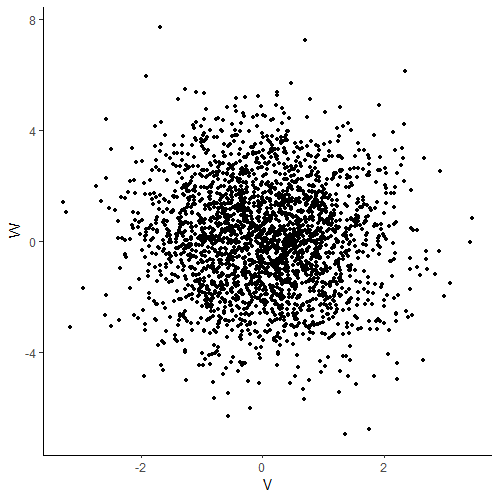
\includegraphics[width=0.9\linewidth]{V_W_Pre.png}
\end{center}
\end{column}
\begin{column}{0.33\linewidth}
\begin{center}
	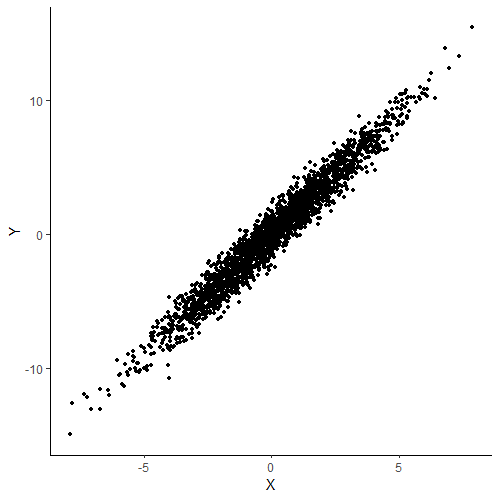
\includegraphics[width=0.9\linewidth]{X_Y_Pre.png}
\end{center}
\end{column}
\begin{column}{0.33\linewidth}
\begin{center}
	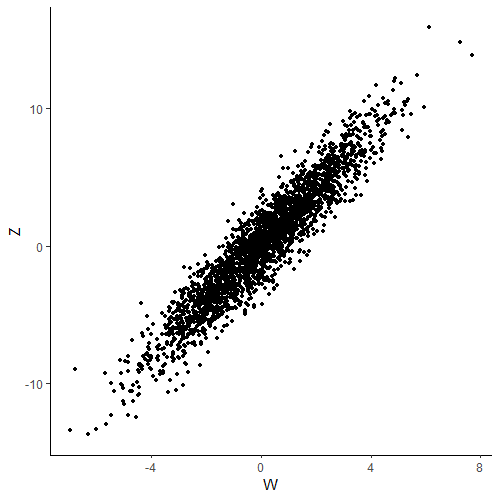
\includegraphics[width=0.9\linewidth]{W_Z_Pre.png}
\end{center}
\end{column}
\end{columns}

\begin{columns}
\begin{column}{0.33\linewidth}
\begin{center}
	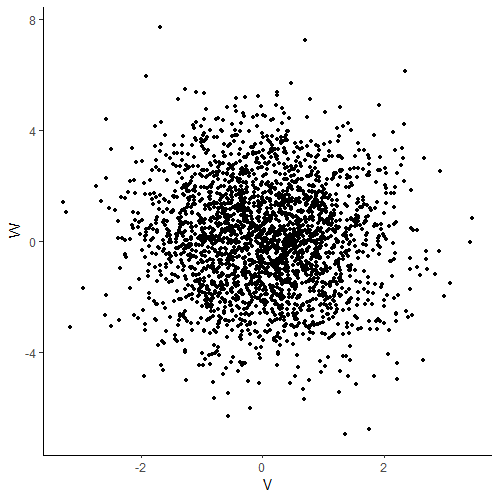
\includegraphics[width=0.9\linewidth]{V_W_Post.png}
\end{center}
\end{column}
\begin{column}{0.33\linewidth}
\begin{center}
	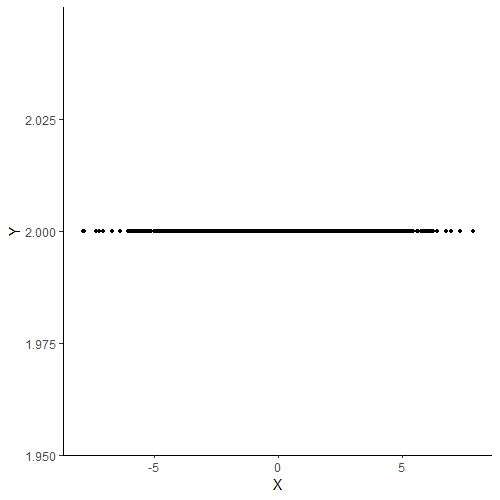
\includegraphics[width=0.9\linewidth]{X_Y_Post.png}
\end{center}
\end{column}
\begin{column}{0.33\linewidth}
\begin{center}
	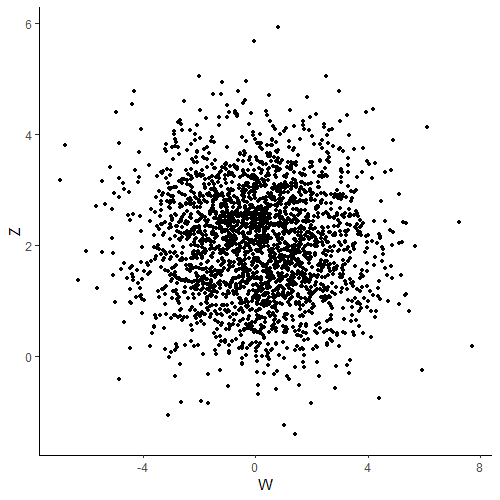
\includegraphics[width=0.9\linewidth]{W_Z_Post.png}
\end{center}
\end{column}
\end{columns}
\end{frame}

\begin{frame}
\frametitle{Normalverteilung}

Man könnte hier jetzt simulieren
\[\mathbb{P}(Z \in [0, 1] \mid \Do(Y = 2)) \approx 14 \%~.\]
\end{frame}

\section{Abgeschnittene Produktregel}

\begin{frame}
\frametitle{Produktdekomposition}

\begin{block}{\textbf{Satz 4.36} \klein{(Produktdekomposition)}}
Sei ein Kausalgraph gegeben und $X_1, \dots, X_n$ alle Variablen in diesem Modell, sowie $x_1, \dots, x_n$ jeweils Werte dieser Zufallsvariablen. Es gilt die folgende \textit{Produktdekomposition}
\[\mathbb{P}(X_1 = x_1, \dots, X_n = x_n) = \prod_{i=1}^n \mathbb{P}(X_i = x_i \mid \Pa(X_i) = \pa(X_i))~.\]
Hierbei sei $\pa(X_i)$ konsistent mit $x_1, \dots, x_n$.
\end{block}
\end{frame}

\begin{frame}
\frametitle{Abgeschnittene Produktregel}

\begin{block}{\textbf{Satz 4.35} \klein{(Abgeschnittene Produktregel)}}
Sei ein Kausalgraph gegeben und $X_1, \dots, X_n$ alle Variablen in diesem Modell, sowie $x_1, \dots, x_n$ jeweils Werte dieser Zufallsvariablen. Sei $X$ eine Zufallsvektor mit Variablen aus dem Modell. Ist $x$ ein Wert des Zufallsvaktors, so gilt die \textit{abgeschnittene Produktregel}
\begin{scriptsize}
\[\mathbb{P}(X_1 = x_1, \dots, X_n = x_n \mid \Do(X = x)) = \prod_{i \in I} \mathbb{P}(X_i = x_i \mid \Pa(X_i) = \pa(X_i))~.\]
\end{scriptsize}
Hierbei sei $I \subset \{1, \dots, n\}$ die Menge aller Indizes der Variablen, die nicht in $X$ sind. Weiter sei $x$ und $\pa(X_i)$ konsistent mit $x_1, \dots, x_n$.\\
Ist dies nicht konsistent, so verschwindet die Interventionswahrscheinlichkeit.
\end{block}
\end{frame}

\begin{frame}
\frametitle{Poissonverteilung}

\begin{center}
\begin{tikzpicture}[->,>=stealth,shorten >=1pt,auto,node distance=2cm,semithick]
  \node (U_X) {$U_X$};
  \node (U_V) [right of=U_X] {$U_V$};
  \node (U_W) [right of=U_V] {$U_W$};
  \node[endo] (X) [below of=U_X] {$X$};
  \node[endo] (V) [below of=U_V] {$V$};
  \node[endo] (W) [below of=U_W] {$W$};
  \node[endo] (Z) [below of=X] {$Z$};
  \node[endo] (Y) [below of=V] {$Y$};
  \node (U_Z) [below of=Z] {$U_Z$};
  \node (U_Y) [below of=Y] {$U_Y$};
  
  \path (U_V) edge node {} (V);
  \path (U_W) edge node {} (W);
  \path (U_X) edge node {} (X);
  \path (U_Y) edge node {} (Y);
  \path (U_Z) edge node {} (Z);
  \path (V) edge node {} (X);
  \path (V) edge node {} (Y);
  \path (W) edge node {} (Y);
  \path (X) edge node {} (Y);
  \path (X) edge node {} (Z);
  \path (Y) edge node {} (Z);
\end{tikzpicture}
\end{center}
\end{frame}

\section{Probleme}

\begin{frame}
\frametitle{Probleme}

\begin{enumerate}[label = (\roman*)]
\item Lokalität
\item Nicht-manipulierbare Variablen
\item Azyklizität
\item Interpretation der Assoziationen
\item Kausalgraph
\item Ungemessene Variablen
\item[(viii)] Verstetigung 
\end{enumerate}
\end{frame}
\end{document}
